\chapter{Implementation} \label{ch:impl}

This chapter will describe the implementation of the system and will serve as an introduction for future developers.

The \SB is implemented as a plugin for the Eclipse workbench. It depends on several other MEVSS plugins which provide 
the AST classes and infrastructure for building the SDG, as well as an Eclipse editor for viewing IEC files. The \SB 
plugin provides two views (the \emph{\SB} view and the \emph{Instance Hierarchy} view) and contributes items to the IEC 
editor context menu.

The plugin is implemented largely in a \emph{model-view-controller} (MVC) pattern, with the model being a use case 
which contains a so-called \emph{display graph}; the display graph wraps the SDG to adapt it to the view and to augment 
it with artificial elements. Since the Eclipse view is currently a singleton view, it instantiates the controller when 
it is shown. The controller instantiates a model when it is asked to display a certain use case, it also keeps a 
history of previous models so the user can navigate between them.


\section{Overview}

This section will give an overview of the packages containing the \SB code and introduce important terminology along 
the way. All packages are part of a common root package \lstinline|at.jku.mevss.featureide.browserview|. The root 
package contains the \lstinline|DependencyBrowserPlugin| class, which represents the plugin instance and provides 
methods for showing AST and SDG nodes in the IEC editor. Also part of the root package is the 
\lstinline|DependencyBrowserController| class, which is the main entry point into the \SB, as well as the 
\lstinline|SDGBrowserSourceProvider| class, which makes the current model available across the workbench.

\begin{description}
  \lstitem{model2} This package contains the use cases which derive from the \lstinline|AbstractModel| base class. A 
  concrete use case is implemented by deriving from that base class and providing strategies for selecting nodes and 
  edges to be displayed. The \lstinline|AbstractModel| instance then builds a \emph{display graph} based on these 
  strategies.
  
  \lstitem{model2.graph} Classes in this package represent the \emph{display graph}, the model that abstracts from the 
  underlying SDG and allows the addition of container nodes (for representing hierarchy) and artificial graph elements. 
  This abstraction also allows the \SB to work with different SDG types without having to change the view 
  implementation. All nodes in the display graph can be in an \emph{expanded} or \emph{collapsed} state, meaning that 
  their logical successors will be shown or hidden, respectively. Furthermore, container nodes can be \emph{closed} so 
  their children are hidden to reduce visual clutter.
  
  All display graph elements derive from the common base class \lstinline|DisplayElement| which provides support for 
  attaching arbitrary properties. Classes \lstinline|DisplayNode| and \lstinline|DisplayEdge| represent nodes and 
  edges, respectively, and also store layout information (position, size, bend points). The \lstinline|DisplayGraph| 
  class stores all nodes and edges representing the graph and provides support for adding new elements. This class also 
  produces graph change events and provides a means for getting the visible part of the graph (elements 
  \emph{reachable} through expanded nodes).
  
  \lstitem{model2.hierarchy} The instance hierarchy is represented by the \lstinline|HierarchyTree| and 
  \lstinline|HierarchyTreeNode| classes in this package. Every \lstinline|AbstractModel| exposes an instance hierarchy 
  tree for its current graph contents.
  
  \lstitem{model2.layout} This package defines the classes used for the graph layout. The only implementation of 
  interface \lstinline|GraphLayouter| is \lstinline|KLayLayouter|, which uses the \emph{KLay Layered}\footnotemark{} 
  layout algorithm.
  
  \footnotetext{KLay Layered is a layer-based layout algorithm and part of the 
  \href{https://rtsys.informatik.uni-kiel.de/confluence/}{KIELER project}, it is currently being integrated into 
  Eclipse as part of the \href{http://www.eclipse.org/elk}{Eclipse Layout Kernel (ELK)}. For more information on KLay 
  Layered see \url{https://rtsys.informatik.uni-kiel.de/confluence/display/KIELER/KLay+Layered} and 
  \cite{DBLP:journals/vlc/SchulzeSH14}.}
  
  \lstitem{event} This package defines listener interfaces and event objects for several events: view changes (a new 
  model being displayed), selection of a node in the view, changes to a \lstinline|DisplayGraph|, and changes to 
  \lstinline|AbstractModel| properties.
  
  \lstitem{command} This package contains classes for interfacing an editor selection (path and source code range) with 
  the \SB controller, as well as the class \lstinline|SDGBrowserCommand|, which represents a command that operates on 
  display graph elements. Subpackage \lstinline|eclipse| defines Eclipse command handlers that plug into the IEC editor 
  context menu, subpackage \lstinline|pipe| defines handlers that receive commands via a Windows named pipe.
  
  \lstitem{command.feature} The interfaces in this package allow an arbitrary graph to be displayed in the \SB by 
  providing a \emph{feature} which may contain a number of \emph{slices} (sets of nodes to include in the graph). This 
  will be used by the FORCE platform~\cite{HinterreiterDA} to display a graph of those parts of the program that belong 
  to a certain feature.
  
  \lstitem{views} This package contains the views contributed to the Eclipse workbench. Class 
  \lstinline|InstanceHierarchyView| and supporting classes implement the \emph{Instance Hierarchy} view, which displays 
  the current model's hierarchy tree. The \lstinline|BrowserView| interface is used by the controller to render a 
  display graph and is partially implemented by the \lstinline|AbstractBrowserView| base class. This class is an 
  Eclipse \emph{view part} that provides several controls for setting model properties, but does not implement graph 
  rendering itself.
  
  \lstitem{views.draw2d} This package and its subpackages contain the classes which implement the 
  \lstinline|BrowserView| interface using Draw2D\footnotemark{}. The implementation class \lstinline|Draw2DBrowserView| 
  extends \lstinline|AbstractBrowserView| and uses the \lstinline|GraphCanvas| class for rendering a display graph. The 
  \lstinline|Resources| class exposes all the colors and dimensions used for the displayed graph elements via static 
  methods, so its implementation may be changed in the future to allow Eclipse settings to be taken into account.
  
  \footnotetext{\href{https://www.eclipse.org/gef/draw2d/}{Draw2D} is a lightweight rendering toolkit on top of SWT, 
  the UI toolkit used by Eclipse.}
  
  The \lstinline|GraphCanvas| class implements most of the heavy lifting to support transitions when graph elements 
  enter or exit, implements zooming and hit testing, and handles events on displayed graph figures. The 
  \lstinline|animation| subpackage contains classes for supporting animations of Draw2D figures; the 
  \lstinline|overview| and \lstinline|tooltip| packages implement the scrollable overview thumbnail and tooltip 
  controls, respectively; all figures and decorations used for rendering are part of the \lstinline|figures| package.
\end{description}


\section{Model}

The model part of the MVC architecture is mainly split in two parts, the display graph and the use cases. Each use case 
is represented by a class which inherits from \lstinline|AbstractModel| and implements strategies for adding elements 
to the graph when nodes are expanded by the user. Each model instance creates a display graph and populates it 
according to the implemented strategy.

An overview of the model classes can be found in the class diagram in \autoref{fig:classes-model}, it shows roughly 
what the structure of a model looks like. The subclasses of \lstinline|AbstractModel|, \lstinline|DisplayNode|, and 
\lstinline|DisplayEdge| are not shown and will be introduced in detail later on.

\begin{figure}[htb]
  \centering
    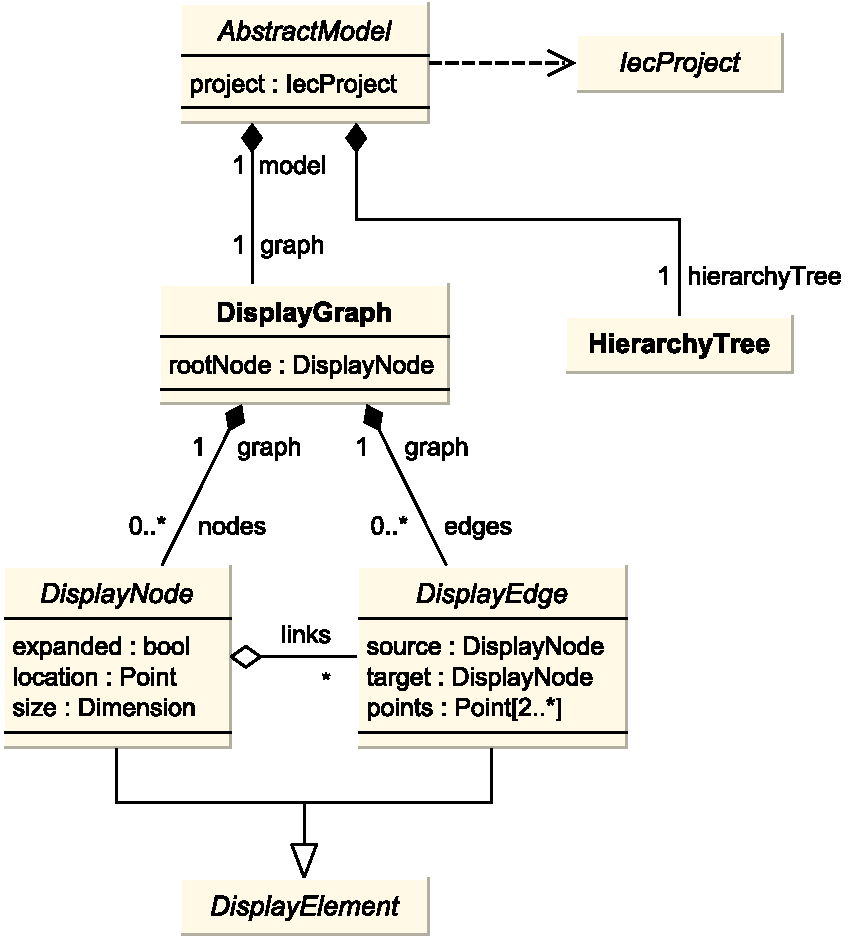
\includegraphics[scale=0.6]{bilder/classes-model}
  \caption{Class diagram overview of the model classes}
  \label{fig:classes-model}
\end{figure}

The \SB uses build infrastructure provided by an Eclipse plugin for viewing IEC files, which was developed in the 
course of Alois Mühleder's bachelor thesis \cite{MuehlederBA} at the CDL MEVSS. The plugin is used to build the SDG 
from an IEC project and also provides ways to navigate the IEC code (\emph{Open Declaration}, search for IEC 
elements like types and variables). The \lstinline|IecProject| interface is part of that plugin and provides access to 
the AST and SDG after a build is completed.

\subsection{Display Graph}

As mentioned in the overview, the display graph is a model that wraps the SDG and abstracts from it to provide a 
uniform interface for the view to use.

Class \lstinline|DisplayGraph| contains alls nodes and edges and maintains maps from keys to nodes and edges, 
respectively. Keys are objects that identify a graph element uniquely and are used to determine whether a node or edge 
is in the graph. For example, a \lstinline|DGDisplayNode| is uniquely identified by the \lstinline|DGNode| it wraps, so 
that is its key; a \lstinline|VariableDisplayNode| is uniquely identified by a \lstinline|DataDefinition| (the AST node 
representing the local variable) and the containing SDG procedure node, so its key is a tuple of those two objects. 
Furthermore, each display graph has one root node, which is the entry point of the graph (the code element being 
investigated, or a group thereof).

The \lstinline|DisplayGraph| class also provides methods for adding new nodes to the graph, instances of node classes 
are created internally as they are needed. This encapsulates creation of new nodes to make sure they are initialized 
only once and to make sure there is only one instance of a node for a particular key; in case a node already exists in 
the graph it is just returned. Edges are added to the graph only through nodes, which provide different methods to add 
edges, depending on the node type. Since every edge in the graph is owned by a node there is no way to add edges to the 
graph directly.

Finally, class \lstinline|DisplayGraph| provides method \lstinline|collectReachableGraph|, together with various 
convenience methods wrapping it, which allows the currently reachable nodes and edges in the graph to be collected into 
provided sets. A predicate may also be specified which is used to filter nodes and edges to be collected. A node in the 
graph is reachable, if there is a path to it from the root node through expanded nodes only (over edges that are not 
filtered).

Both display graph nodes and edges inherit from the abstract class \lstinline|DisplayElement|. This class declares 
several abstract methods that all display element need to implement, two of which are \lstinline|getKey()| and 
\lstinline|accept(GraphVisitor<T>)|. The former returns the unique key for any graph element, the latter is 
implemented in every leaf class of the hierarchy and implements the visitor pattern for graph elements. Furthermore, 
class \lstinline|DisplayElement| provides support for properties and tooltip data. Properties are used to store 
arbitrary information with a graph element, for example whether a node is flagged or hidden, but is not meant to be 
viewed by the user. Tooltip data, on the other hand, is meant to be shown to users in a tooltip for any graph element.

\subsubsection{Nodes}

A diagram showing all classes of display graph nodes can be seen in \autoref{fig:classes-displaynode}. Abstract class 
\lstinline|DisplayNode| represents a node in the graph. It stores layout information (location and size), a set of 
links (edges owned by the node), the parent node, and whether or not the node is expanded. It also defines abstract 
methods \lstinline|getName()| and \lstinline|getType()| for the view.

\begin{sidewaysfigure}[p]
  \centering
    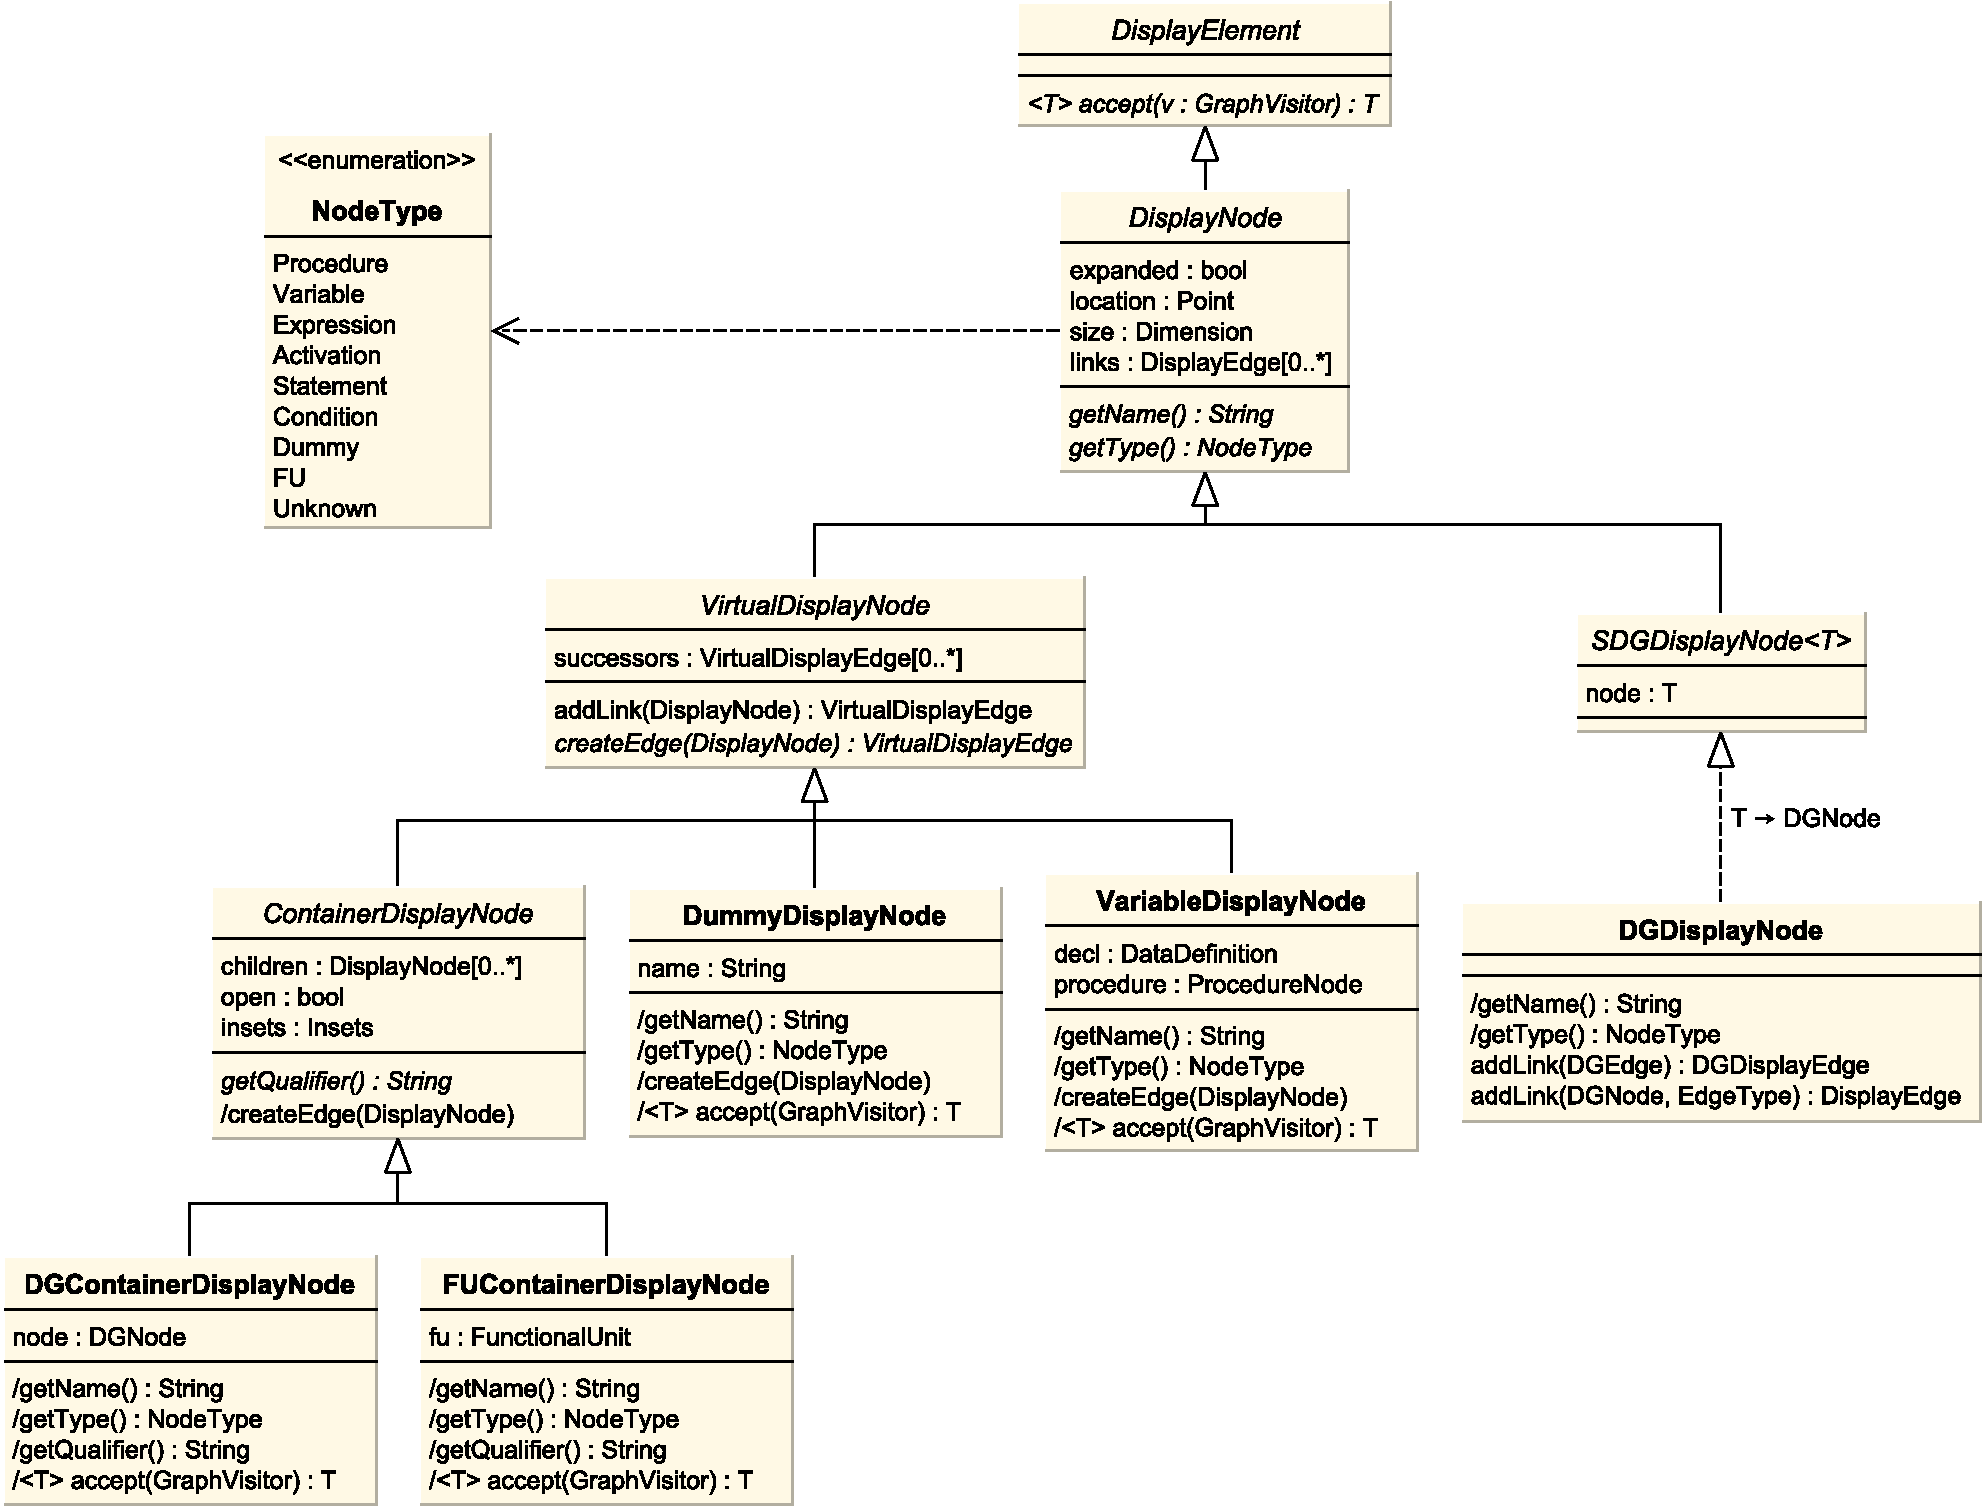
\includegraphics[scale=0.5]{bilder/classes-displaynode}
  \caption{Class hierarchy of display graph nodes}
  \label{fig:classes-displaynode}
\end{sidewaysfigure}

\lstinline|DisplayNode| has two abstract subclasses: \lstinline|VirtualDisplayNode| represents an artificial node that 
has no corresponding SDG node; \lstinline|SDGDisplayNode| represents a node backed by an actual SDG node. The abstract 
class \lstinline|ContainerDisplayNode| represents a container for other node, it adds insets for the layout and stores 
a set of child nodes.

The only subclass of \lstinline|SDGDisplayNode| at the moment is \lstinline|DGDisplayNode|, which is backed by a 
\lstinline|DGNode|. It implements \lstinline|getName()| and \lstinline|getType()| in terms of utility methods provided 
by class \lstinline|GraphUtil|. To add support for other SDG types, alternatives need to be added for three classes 
only: \lstinline|DGDisplayNode|, \lstinline|DGContainerDisplayNode|, and \lstinline|VariableDisplayNode|. The latter 
could instead be changed to store the procedure instance using \lstinline|AstmInstance| instead of a procedure node.

\subsubsection{Edges}

A diagram showing all classes of display graph edges can be seen in \autoref{fig:classes-displayedge}. Abstract class 
\lstinline|DisplayEdge| represents an edge in the graph. It stores the source and target display nodes and layout 
information (start and end points, optional bend points). It also defines the abstract method \lstinline|getType()| for 
the view.

\begin{sidewaysfigure}[p]
  \centering
    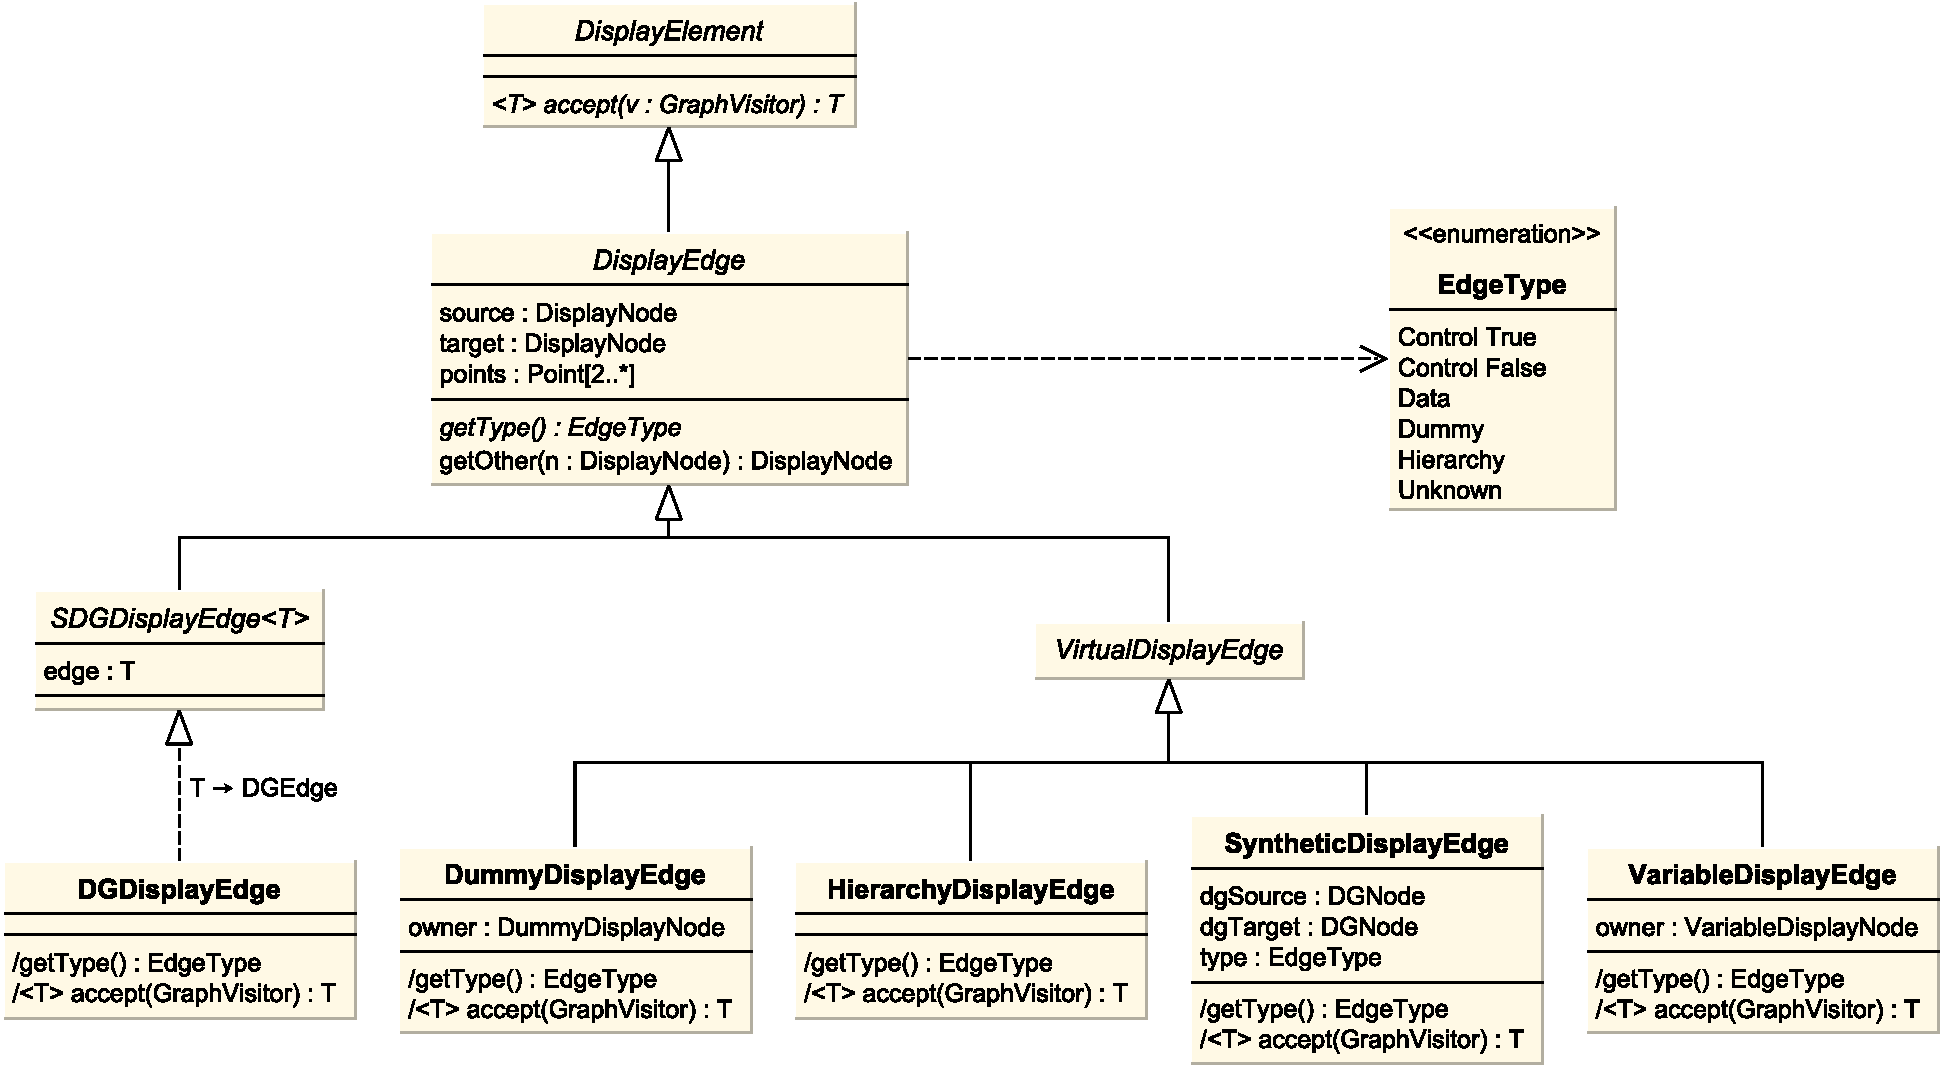
\includegraphics[scale=0.5]{bilder/classes-displayedge}
  \caption{Class hierarchy of display graph edges}
  \label{fig:classes-displayedge}
\end{sidewaysfigure}

\lstinline|DisplayEdge| has two abstract subclasses: \lstinline|VirtualDisplayEdge| represents an artificial edge that 
has no corresponding SDG edge; \lstinline|SDGDisplayEdge| represents an edge backed by an actual SDG edge.

The only subclass of \lstinline|SDGDisplayEdge| at the moment is \lstinline|DGDisplayEdge|, which is backed by a 
\lstinline|DGEdge|. To add support for other SDG types, alternatives need to be added for two additional classes 
only: \lstinline|DGDisplayEdge|, and \lstinline|SyntheticDisplayEdge|. The latter connects two arbitrary 
\lstinline|DGNode|s and only needs an alternative in case such edges should exist for nodes in the new SDG as well.

Links are added to the graph via the protected method \lstinline|addLink| provided by class \lstinline|DisplayNode|. 
Subclasses of \lstinline|DisplayNode| may provide concrete methods for creating edges from SDG edges or for creating 
artificial edges.

\subsection{Use Cases}

Use cases are implemented as concrete classes derived from \lstinline|AbstractModel|. This class contains the display 
graph and instance tree and maintains properties which are used to store the view configuration (e.g.\ whether flagged 
nodes are hidden). The abstract method \lstinline|getType()| must be implemented by concrete use cases and gets the 
name of the use case (i.e.\ the type of model). \autoref{fig:classes-usecase} shows a diagram of all model classes.

\begin{figure}[htb]
  \centering
    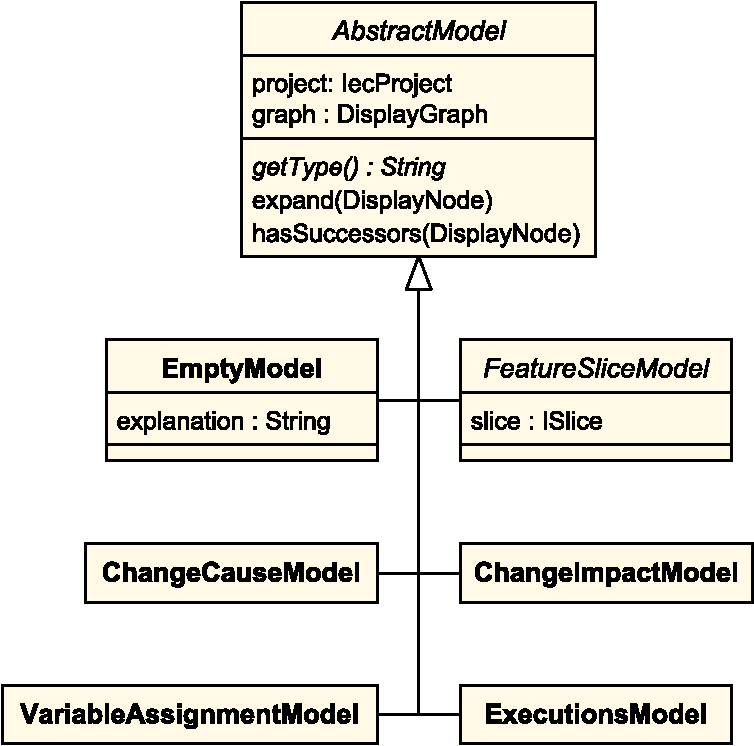
\includegraphics[scale=0.5]{bilder/classes-usecase}
  \caption{Class hierarchy of use cases}
  \label{fig:classes-usecase}
\end{figure}

The two most important methods in the \lstinline|AbstractModel| class, which implement a model's strategy for adding 
successors of a node to the graph when it is expanded, are \lstinline|hasSuccessors(DisplayNode)| and 
\lstinline|expand(DisplayNode)|. Their default implementations delegate to overloads for concrete display node types, 
subclasses need only implement (some of) them, depending on what types of nodes are created.

There are two model classes which do not correspond to one of the use cases defined in \autoref{ch:usecases}: 
\lstinline|EmptyModel| and \lstinline|FeatureSliceModel|. The empty model is used whenever there are no instances of a 
selection, or if a feature slice is empty, and contains one dummy node with an explanation. Class 
\lstinline|FeatureSliceModel| is used to display an \lstinline|ISlice|, which is basically an arbitrary set of SDG 
nodes. The current implementations of forward and backward slice models only follow control edges.

%When a model is first created (which typically happens in factory methods) its graph must be populated with at least 
%one node (the root node). In the case of multiple root nodes, a dummy node is used to group them.
The other four \lstinline|AbstractModel| subclasses each implement one concrete use case of the \SB. They each override 
only those methods for node types which actually occur in the graph, for example \lstinline|ExecutionsModel| never 
creates any variable nodes so it doesn't overload \lstinline|hasSuccessors| and \lstinline|expand| for those nodes.

The view uses \lstinline|hasSuccessors| to determine whether a node can be expanded to indicate this to the user. It 
should follow the same logic as \lstinline|expand| so the view is consistent with the model semantics. Nodes are added 
to the graph in the \lstinline|expand| method; whenever a user clicks on a node this method is called to add successors 
of the clicked node to the graph.


\section{Controller}

TODO


\section{View}

TODO

\subsection{Eclipse View Part}

TODO

\subsection{Draw2D View}

TODO


\section{Commands}

TODO


\section{Future Work}

TODO
